\chapter{Evacuation planning: towards an integrated approach}
\label{ch:evacuation}
% ##################################################################################################################

\hfill \textbf{Author:} Gregor L\"ammel, Christoph Dobler, Hubert Kl\"upfel 

% add a meaningful figure here.
\begin{center} 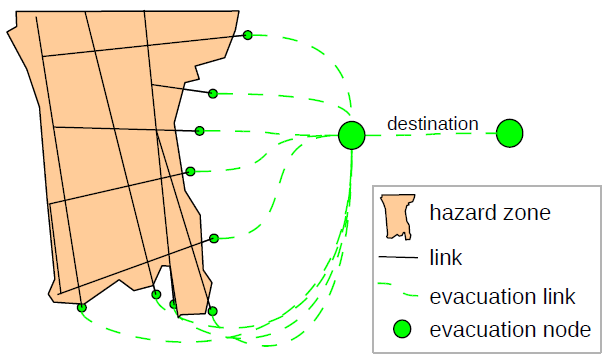
\includegraphics[width=0.4\textwidth, angle=0]{extending/figures/Evacuation/evacuation} \end{center}

This chapter presents an integrated approach for performing evacuation simulations with MATSim.
This integrated approach comprises all steps of the workflow for performing an evacuation analysis, i.e., 
selecting the evacuation area and defining the population, specifiying the behavioral parameters 
(i.e. the pre-movement time distribution and the mode of evacuation - car or pedestrian), 
and analysing the simulation output.
These steps can all be performed within one graphical user interface.
Additionally, two extensions of MATsim for simulating public transport and for changing the network 
during the simulation (i.e. network change events) are accessible from the GUI.
In this chapter the steps for performing such an integrated analysis are described and illustrated based on
the example of Hamburg-Wilhelmsburg.

\section{Related work}
\hl{TODO: give references to existing work MATSim related work (e.g.  Diss, Dobler within-day evacuation ...?).
References to other work in the evacuation context are given in Laemmel's Diss - needs to be updated, however.}
Additional work related to evacuation simulations in MATSim is presented by \citet{Dobler_PhDThesis_2013}. The main difference to the approach presented in this chapter is that agents are allowed to adapt their plans on-the-fly using MATSim's within-day replanning framework \citep{DoblerEtAl_TRR_2012}. 
Based on a behavioral model, agents coordinate their actions on household level. If a household is e.g. not joined when the evacuation starts, each member estimates the time to return home as well as the time to leave the evacuation area directly. Then, the household decides whether meeting at home and leaving together is preferred over every member leaving on its one.
Since the behavioral model is implemented on agent respectively household level, individual attributes such as presence of children in the household or availability of a car can be taken into account.
In contrast to regular MATSim simulations, only a single iteration is performed. Since the agents can optimize their plans continuously using real time information, no further replanning is necessary. As a result, it is guaranteed that agents do not foresee future events such as traffic jams caused by people leaving the threatened area.


%\section{Integrated modeling approach for rapid evacuation planning}
%\hl{TODO: short introduction to GRIPS}
%\section{Input data}
%\hl{TODO: discribe what is needed, where one may get it from, and how it has to transform (if needed).}
%\begin{itemize}
%\item osm file
%\item grips config
%\end{itemize}

\section{Download Matsim and Grips}
\begin{enumerate}
\item 
Download the current nightly build of Matsim and Grips from
\url{http://matsim.org/files/builds/}
\item 
Unzip the \verb|Matsim_rxxxxx.zip|, \verb|Matsim_libs.zip| and\\
 \verb|grips-0.6.0-SNAPSHOT-rxxxxx.zip|.
\item 
Move the \verb|grips-0.6.0-SNAPSHOT-rxxxxx.jar| and \verb|libs| folder from the \verb|grips-0.6.0-SNAPSHOT-rxxxxx| directory one level up, 
i.e., to the directory, where \verb|MATSim_rxxxxx.jar| is located.
\end{enumerate}

You can test your configuration by invoking\\ 
\verb|java -cp grips-0.6.0-SNAPSHOT.jar;MATSim_rxxxxx.jar|\\ \verb|org.matsim.contrib.grips.scenariomanager.ScenarioManager|.\\
(You might also want to copy that command to a file \verb|grips.bat| -- or \verb|grips.sh| if using a Unix-like operation system. You can then run that file instead of typing the command.)

\section{The fifteen minute tour}\label{evac:section:fifteenminute}
If you just want to get a quick impression, then the following steps can be performed within a few minutes:
\begin{description}
\item[OSM] Go to \url{www.openstreetmap.org} search for your favorite place and download a (small) osm. Please choose a small area, e.g. 100m by 100m. This is sufficient for the beginning and the size of the exported area is limited. For larger areas, a direct download from sites like \url{www.geofabrik.de} is preferable (see next section).
\item[Run] the ScenarioManager as described in the previous section.
\item[Create] a scenario by clicking the leftmost button first and then "New". Go to the directory where you'd like to save your project and name the project file (e.g., london.xml or scenario.xml).
\item[Specify] The path of the osm-file (by clicking "Set" next to network), the area ("Set" next to "evacution file") and population files "Set" next to "population file" , and the output directory.
A useful convention is to save everything in the same directory and to name the area file "area.shp" and the population file "population.shp". You can also create sub-directories area and population and save them there.
\textbf{This step has to be done only once. After the scenario-file has been saved, you can just open it in the Scenario-Manager.}
\item[Sample size] Set the sample size to 0.1 (you can use the mouse or the cursor buttons of your keyboard).
\item[Departure] Specify the departure time distribution. Plausible values could be: normal distribution, mu and sigma 600 seconds (10 minutes), earliest 300 seconds, latest 1200 seconds (20 minutes).
\item[Save] your scenario file.
\item[Create] area.shp and population.shp. Currently, the area.shp and population.shp must exist before switching to the area tab. You can download and unzip \url{www.traffgo-ht.com/download/research/grips/shp.zip}. Please make sure all the area and population files (shp, dbf, and some others) are stored in the directory specified in the scenario-file.
\item[Area] Switch to the area tab. You can define the circular evacuation area by keeping the left mouse button pressed and defining the center and radius. Don't forget to save your changes.
\item[Population] Switch to the population tab and define the population (handling is similar to area). Don't forget to save your changes.
\item[Convert] Switch to the next tab and convert the scenario to MATSim input files by clicking the "run" button. The MATSim files will be stored in the output directory specified in the beginning.
\item[Run] the MATSim simulation by skipping the next two tabs/buttons (road closures and busses) and switching to the simulation tab (with the little M for MATSim on the computer screen). Click "run". This will take a while.
\textbf{The output directory will be overwritten. If you want to keep previous results, please rename the output directory.}
\item[Analyze] your simulation results by switching to the final tab after the simulation is finished.

\end{description}

\section{Input data (any place and any size)}
%\hl{TODO: discribe what is needed, where one may get it from, and how it has to transform (if needed).}
The only external input that is necessary for performing an evacuation analysis with \verb|org.matsim.contrib.grips| is an OpenStreetMap file.
You can download OpenStreetMap files from 
\verb+download/geofabrik.de+.
For the sake of this tutorial, we will use the file for Hamburg, Germany. 
Please go to \url{http://download.geofabrik.de/europe/germany/hamburg.html} and download the \verb+hamburg-latest.osm.bz2+ file. This is all the initial preparation you need. Everything else can 
be done with the GUI, called \verb+ScenarioManager+.

\section{Scenario Manager}
\hl{TODO: introduction to Scenario Manager, contrib.grips, what the scenario does and what don't, and how to use it.}

The scenario setup, evacuation simulation, and analysis is handled by the so called \verb+ScenarioManager+.
The \verb+ScenarioManager+ is part of the MATSim contribution package \verb+org.matsim.contrib.grips+, where \verb+grips+ stands for GIS-based Risk-Analysis-, Information-, and Planning-System for Regional Evacuation.
The \verb+ScenarioManager+ manages several modules that constitute a tool-chain ...

\subsection{Scenario configuration}


 At start-up the \verb+ScenarioManager+ offers the opportunity to either defining a new scenario configuration or opening an existing one from a XML-file (which then subsequently can be modified). Figure~\ref{chap:evac:fig:sc_man} shows a screen shot of a scenario configuration in the \verb+ScenarioManager+ and the corresponding XML-file respective.

\begin{figure}[!ht]
\begin{subfigure}
\centering
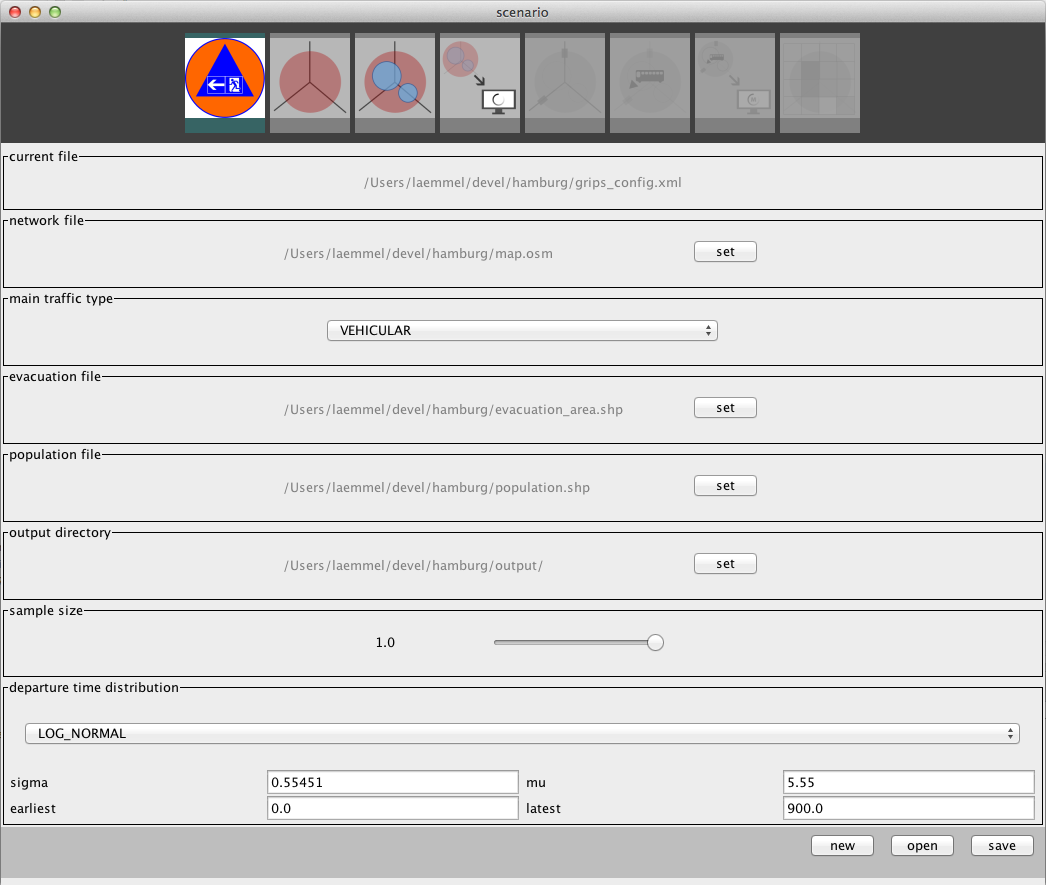
\includegraphics[width=.475\linewidth]{extending/figures/Evacuation/grips_config}
\end{subfigure}\hfill
\begin{subfigure}
\centering
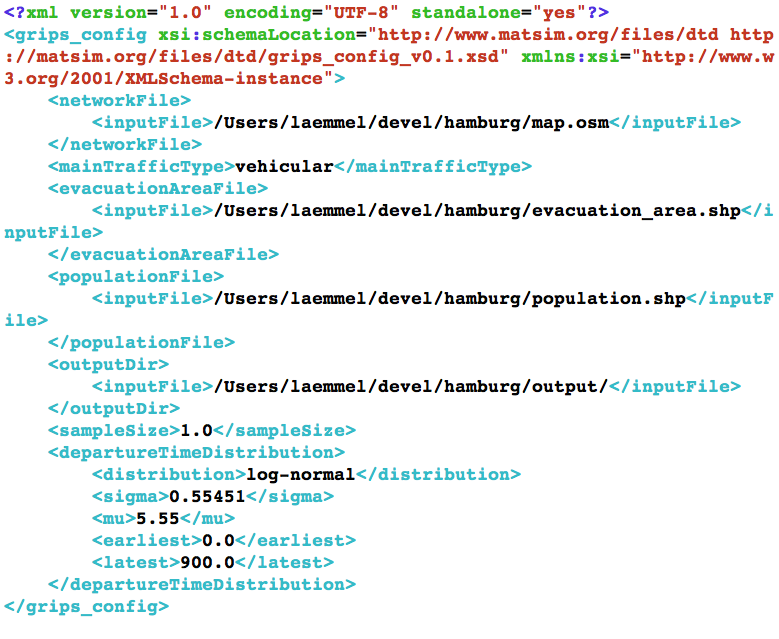
\includegraphics[width=.475\linewidth]{extending/figures/Evacuation/grips_config_xml}
\end{subfigure}
\caption{Illustration of a configurarion opened in the \mbox{ScenarioManager} (left) and as XML-file (right).}\label{chap:evac:fig:sc_man}
\end{figure}
The following parameters have to be specified:
\begin{itemize}
\item The path to the network file for the evacuation scenario. Currently only openstreetmap XML-files are supported (*.osm).
\item The main traffic type for the simulation. This can be either \verb+VEHICULAR+ or \verb+PEDESTRIAN+. Depending on the choice a vehicular specific (the MATSim default) or a pedestrian specific (as discussed in~\citet{LaemmelKluepfelNagel2009EvacPadangAtBookTimmermanns,Laemmel2011Diss}) simulation network will be generated by setting free spee, number of lanes, and flow capacity for the links in the network accordingly.
\item The path to an ESRI-Shape file describing the extend of the evacuation area by a simple polygon. This file does not need to be exist right from the beginning but can be produced manually by the \verb+ScenarioManager+ itself as discussed later.
\item The path to an ESRI-Shape file giving the number and distribution of the affected population. This file comprise of a set of simple polygons with each polygon has the number of persons residing inside this polygon as an additional attribute. As for the evacuation area this file can be produced with help of the  \verb+ScenarioManager+.
\item The path to the output directory where the simulation output and MATSim scenario files will be stored.
\item The sample size for the MATSim simulation. A smaller sample size increases the simulation performance, while a larger size might increase accuracy of the results. Typical values are 1.0, 0.1, or 0.01 depending on the scenario and the available computing resources.
\item The departure time distribution defines the distribution from which the departure times for the simulation will be drawn. The intention behind this is that in real evacuation situation it is not expected that everybody starts simultaneously with their evacuation once the evacuation order has been issued. People tent to perform pre-evacuation activities before they start. Those activities include picking up relatives, to pack food, cloths, or valuable belongings, and other things. Since number and duration of those activities differs on the individual level the departure times of the population reflect an unknown departure time distribution. The \verb+ScenarioManager+ supports three different distributions (Dirac-delta, normal, and log-normal). If the user choses the Dirac-delta distribution then all evacuees will start at once, which might be the worst case~\citep{LaemmelKluepfel2012InfluenceOfDepartureTimeDistribution}. By choosing the normal distribution the departure times for the individuals are drawn from a normal distribution with mean $\mu$ and standard deviation $\sigma$, where the parameters $\mu$ and $\sigma$ are of unit [second]. As an example, setting $\mu = 1800$ and $\sigma =  900$ will result in a departure time distribution where on average after 30 min 50\% of the population has departed and 68.3\% of the population departs in the time interval of 30 min $\pm$ 15 min. If the user decides to choose log-normal as the distribution then the departure times are drawn from a log-normal distribution, where $\mu$ and $\sigma$ are the parameters of the associated normal distribution (a discussion on this matter is given below). The parameters \emph{earliest} and \emph{latest} determine the earliest and latest possible departure time. The normal and log-normal departure time distribution are truncated accordingly.
\end{itemize}
The departure time distribution is maybe the most unclear parameter to set. The authors are not aware of any holistic research into this matter. In general it seems to be reasonable to assume that a lot of people starting the evacuation at about the same time soon after the evacuation order has been issued and as the the time proceeds fewer and fewer people still have to depart. This calls for a departure time distribution who's corresponding probability density function has a steep positive gradient at the beginning and after a peak levels out slowly. The probability density function of a log-normal distribution produces this kind of curve. log-normal and normal distributions are closely related. If the random variable $Y$ is normal distributed, then $X = \text{exp}(Y)$ is log-normal distributed. The expected value $E[X]$  and the variance $Var[X]$ are
\begin{equation}
E[X] = \text{exp}(\mu + \frac{\sigma^2}{2})
\end{equation}
and 
\begin{equation}
Var[X]=\text{exp}(2(\mu+\sigma^2))-\text{exp}(2\mu+\sigma^2).
\end{equation}
Conversely, if the expected value and variance is given $\mu$ and $\sigma$ of the associated normal distribution can be obtained as follows:
\begin{equation}
\sigma = \sqrt{\text{log}(1+\frac{Var[X]}{(E[X])^2}}\label{chap:evac:eq:sigma}
\end{equation}
and 
\begin{equation}
\mu = \text{log}(E[X] - \frac{1}{2}\sigma^2).\label{chap:evac:eq:mu}
\end{equation}
If the users wishes to generate a population with departure times that follow a log-normal distribution it is hard to see how $\sigma$ and $\mu$ will determine the outcome. It is much more convenient to think about the expected value and variance. Given Equations~\ref{chap:evac:eq:sigma} and \ref{chap:evac:eq:mu} a conversion from expected value and variance to $\sigma$ and $\mu$ is straightforward.

\subsection{Evacuation area}% and population}
The \verb+ScenarioManager+ integrates modules for the definition of the evacuation area and the distribution of the affected population. The so called evacuation area selection module allows the user to define the evacuation area by drawing either a simple polygon or a circle on map. The application can make use of either a WMS-provider or a tile map provider (e.g. openstreetmap) as background map renderer. Zooming and panning is restricted to the bounding box of the openstreetmap network file provided in the scenario configuration. An illustration of the evacuation area selector is given in Figure~\ref{chap:evac:fig:area_pop}. Besides defining a new evacuation area a pre-existing one can also be loaded into the \verb+ScenarioManager+. The requirements to a pre-existing evacuation area file are:
\begin{itemize}
\item It has to be provided as a ESRI-Shape file.
\item The evacuation area must be defined as a simple polygon or a multi-polygon that exist of one and only one simple polygon.
\item The coordinate reference system for polygon in the ESRI-Shape file has to be set correctly. 
\end{itemize}
However, due to the error-proneness of this approach it is only recommended for experienced users.

Later in the process the \verb+ScenarioManager+ takes the evacuation area to cutout an evacuation network. However, after cutting out the evacuation net there is no particular node as the target of the path
calculation, as the evacuees have more than one safe place to evacuate to. Instead,
in the underlying domain every node outside the evacuation area is a possible
destination for an evacuee that is looking for an escape route. Thus the evacuation problem is in general a multi-destination problem. To resolve this,
the standard approach (e.g.~\citet{FordFulkerson1962FlowsInNetworks,LuGeorgeEtAl2005CapacityConstrainedRouting})
is to extend the network in the following way: All exit links (i.e.\ links that are originating inside the evacuation area and terminating outside the evacuation area) are connected, using virtual links with infinite flow capacity
and zero length, to a super-node, and all evacuation paths are routed to the super-node. This way, the problem is reduced to a multi-source single-destination problem. And thus, finding the shortest path from any node inside the evacuation area to this super-node and, in consequence, to safety is efficiently to solve.


\subsection{Evacuation demand}
The approach to define population distribution is similar to that of the evacuation area. The difference is that the population is distributed over circles drawn on the map. The use may draw an arbitrary number of those circles and define for each circle the population figures individually. Figure~\ref{chap:evac:fig:area_pop} illustrates the population editor. 
\begin{figure}[!ht]
\begin{subfigure}
\centering
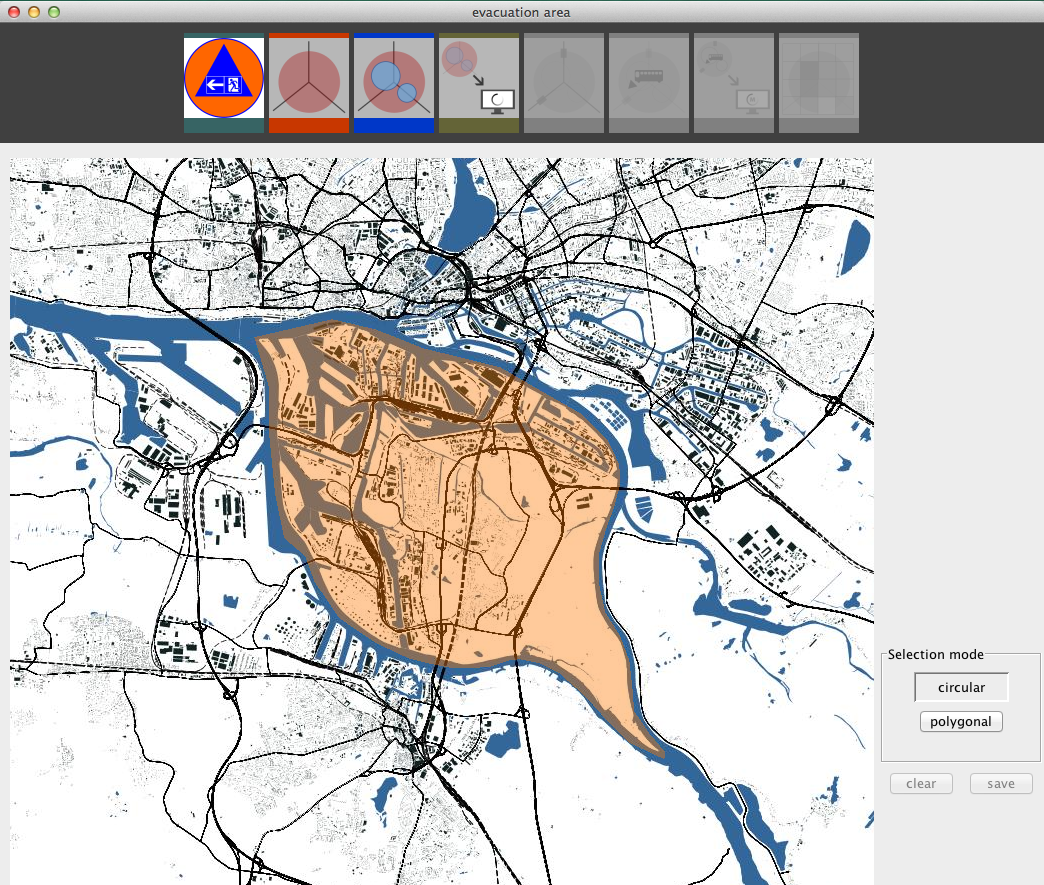
\includegraphics[width=.475\linewidth]{extending/figures/Evacuation/evac_area_sel}
\end{subfigure}\hfill
\begin{subfigure}
\centering
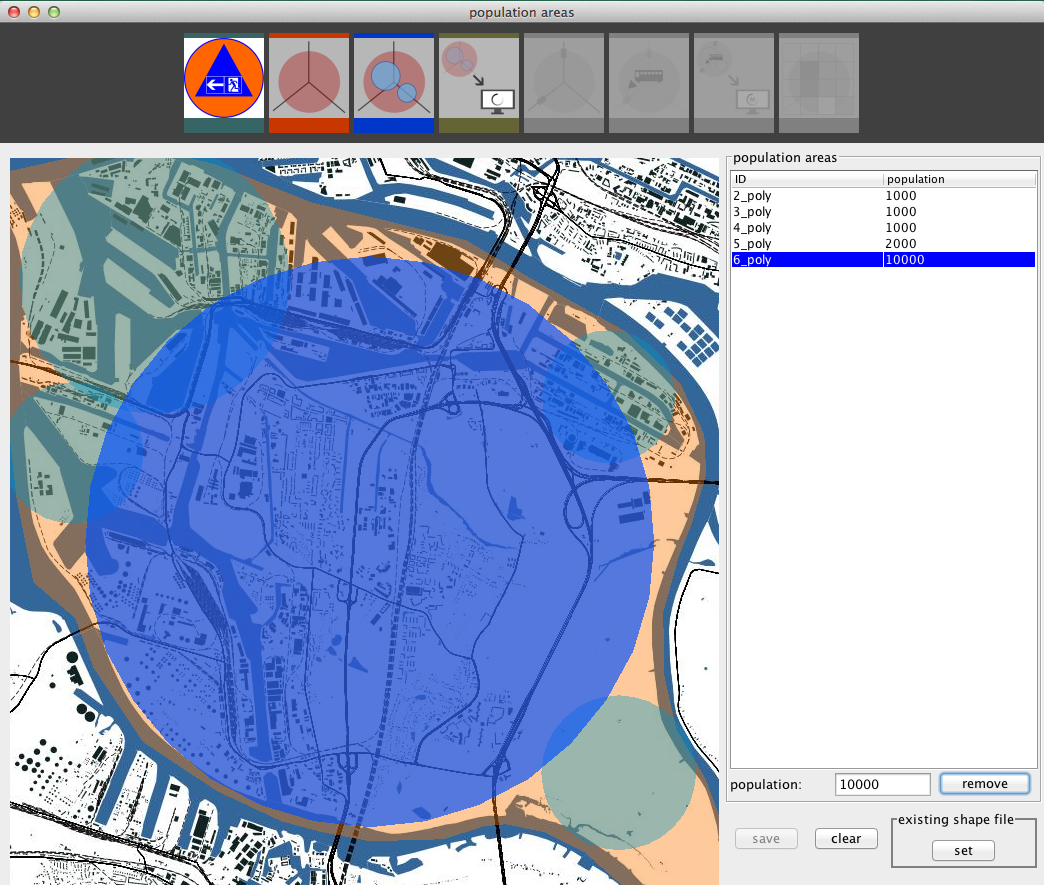
\includegraphics[width=.475\linewidth]{extending/figures/Evacuation/pop_sel}
\end{subfigure}
\caption{The evacuation area (left) and the population distribution (right) can be defined with an integrated GIS application.}\label{chap:evac:fig:area_pop}
\end{figure}
The population editor only offers basic functionality to define a population distribution. For every circular area the \verb+ScenarioManager+ produces as many agent as requested and assigns for each agent a random coordinate inside the circular area. However, in MATSim agents depart on links so the \verb+ScenarioManager+ calls the \verb+getNearestLink()+ method defined in \verb+NetworkImpl+. Thus, agents will depart on links inside and possibly nearby the circular areas. 

In the current version it is not possible to use a predefined demand for the simulation. Extending the simulation package in this way would be straightforward but is out of scope of this work.


\subsection{Road closures}
In a real evacuation situation it is often the case that not all exiting roads can be used. This might be for several reasons:
\begin{itemize}
\item They might be impassable due to the event. This is often the case in flooding related evacuations.
\item The authorities might want to keep roads open exclusively for rescue forces.
\item In some situations, like hurricane evacuations, the direction of lanes on motorways might be reversed to in crease the flow capacity in one direction.
\item The authorities have detailed evacuation plans in place with pre-planned evacuation routes and so road closures might become necessary in order to force evacuees of taking this routes.
\end{itemize}
The actual planning of road closures can be a complex undertaking and not all attributes of such a planning can be regarded in a simple tool for rapid evacuation planning. Nevertheless, the  \verb+ScenarioManager+ offers a tool for editing of time-dependent road closures. An illustration of the road closures editor is given in Figure~\ref{chap:evac:fig:rd_closures_bus_stops}
\begin{figure}
\begin{subfigure}
\centering
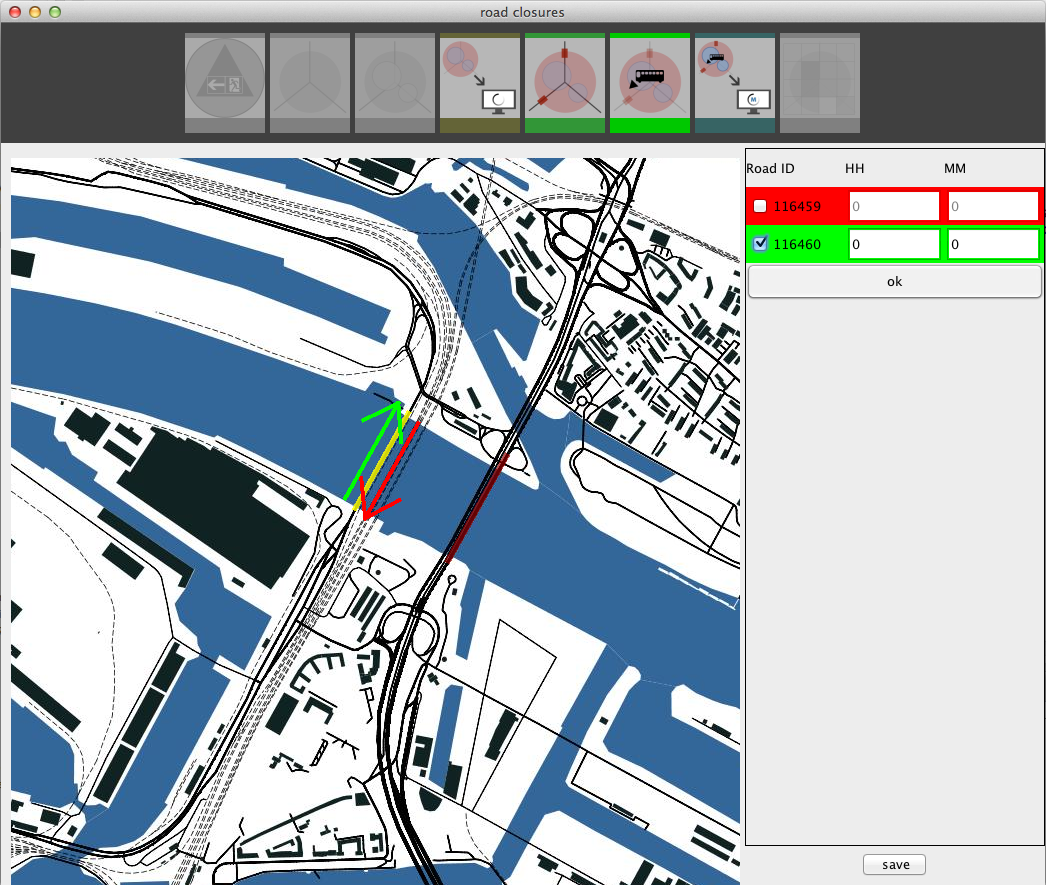
\includegraphics[width=.475\linewidth]{extending/figures/Evacuation/rd_closure_detail}
\end{subfigure}\hfill
\begin{subfigure}
\centering
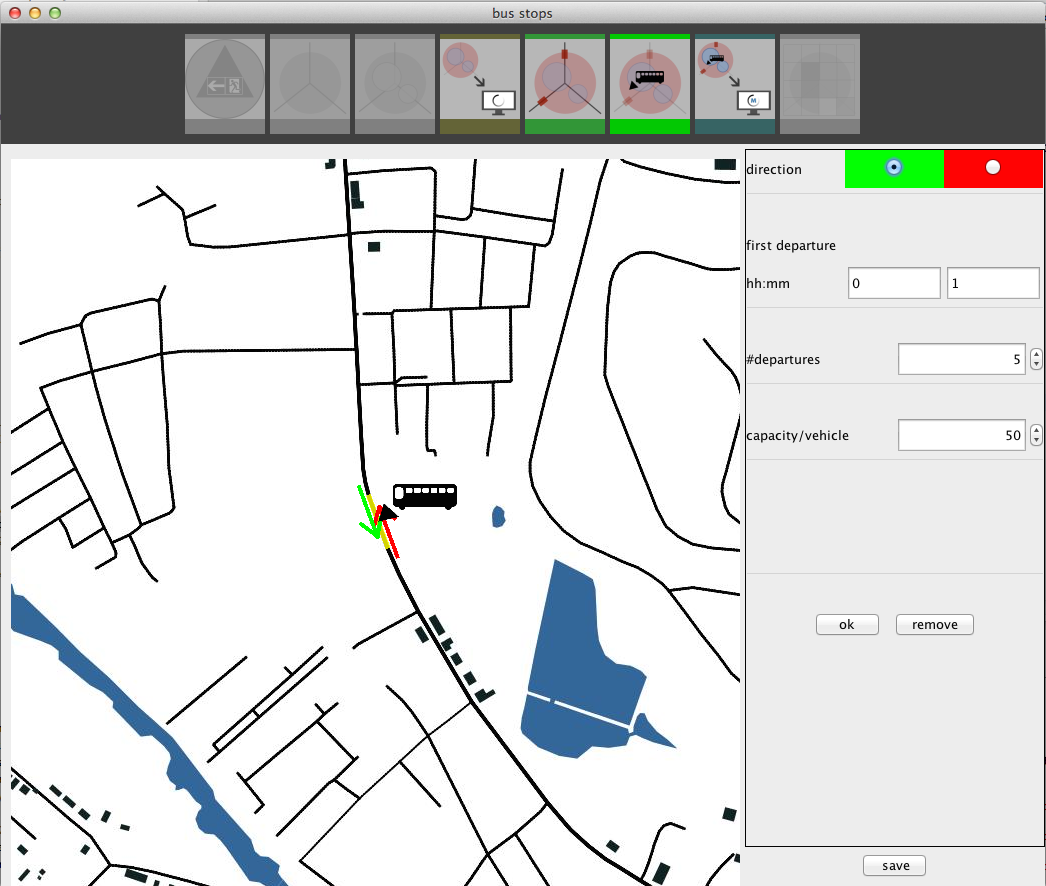
\includegraphics[width=.475\linewidth]{extending/figures/Evacuation/bus_stops}
\end{subfigure}
\caption{Left: Road closures can be edited by an integrated GIS application. For every link the direction and the time of closure can be defined. Right: Tool that let the user define bus stop locations and schedules }\label{chap:evac:fig:rd_closures_bus_stops}
\end{figure}
Road closures are stored as \verb+NetworkChangeEvents+ and handled as time-dependent network attributes in MATSim.

\subsection{Bus stop editor}
Usually not all people have access to a private vehicle. In the event of an evacuation those people often rely on public transport. What is more, in region that are prone for natural disasters the local authorities normally have detailed evacuation plans in place. Those plans might include the evacuation by public transport. Therefore it would be of great interest to integrate the evacuation with public transport into to the simulation framework. The \verb+ScenarioManger+ offers the possibility of defining bus stops and bus schedules for these stops in the interactive GUI. Figure~\ref{chap:evac:fig:rd_closures_bus_stops} gives an example of such a bus stop. Besides the location the user can define when the first bus will serve this bus stop, how many busses overall will serve this particular bus stop and of what capacity those busses are. The \verb+ScenarioManager+ transforms the inputs made in this GUI into a MATSim compatible transport schedule. This means it enriches the scenario uses, however, the same simulation model as before. Details about public transport simulations with MATSim are given here~\citet{TODO}. A tutorial can be found on the MATSim webpage (\verb+http://matsim.org/docs/tutorials/transit+).
Limitations of the public transport evacuation approach in this project are:
\begin{itemize}
\item Each bus serves one and only one bus stop, which might be not too unrealistic either.  
\item Busses alway take the shortest path from their designated bus stops to the safe area. As the shortest path is not necessarily the fastest path this approach might lead to avoidable delays. Some newer research investigate the optimization of bus lines with respect to traffic demand and traffic condition~\citep{Neumann_PhDThesis_2014}. Implementing such optimization techniques int the evacuation context is a topic of future research.
\end{itemize}

\subsection{Running the scenario}
The \verb+ScenarioManager+ runs the evacuation simulation in similar way it is done in other transport simulation studies with MATSim. At the beginning an evacuation plan is assigned to every evacuee. An evacuation plan describes the way how the evacuee intents to reach the safe area. If the an evacuee evacuates by car or foot then such a plan essentially comprise a route (typically the shortest route) from home to the safe area. For evacuees who are evacuating by public transport such a plan can be much more complex. All those evacuation plans will be executed in the mobility simulation. After the mobility simulation terminates all plans are scored regarding their resulting travel time. As shorter a plan's resulting travel time is as high are the score it receives. After this step the evacuees' plans are revised some evacuees will receive new plans while others will stick with the current ones. This step is called re-planning. Mobility simulation, scoring, and re-planning are repeated in a loop for a predefined number of iterations. The evacuees' individual performance improve over the iterations. 
In general transport studies this approach is meant to emulate the real-world travelers behavior when they perform their daily commutes and try to find better travel alternatives. Evacuations, however, are singular events where such a day-to-day re-panning would not occur. We would argue here that the chosen iterative learning approach could be seen as the evacuees anticipation of the conditions that are expected during an evacuation. Since people knowing their  environment would likely avoid roads that obviously constitute bottlenecks during an evacuation. Nevertheless, there is more research needed in order to get a definitive answer how people choose evacuation routes or how many iterations of learning are realistic to reflect the assumed anticipation skills adequately. As a rule of thumb, running 100 iterations of learning are usually enough to get results the constitute a lower boundary in terms of resulting evacuation times.
This is only a rough description of the iterative learning frame work. Details about the general framework are discussed in Chapter~\ref{TODO reference to matsim lerning framework chapter}. Deeper insights into evacuation planning with MATSim can be found in~\citep{Laemmel2011Diss}.

\subsection{Analysis}
After the last iteration has finished the \verb+ScenrioManager+ enables the analysis module. The analysis modele can evaluate the just performed simulation run be a number of different methods. 
\begin{itemize}
\item The evacuation or cumulated arrival curve tells the user the number of evacuated persons over time. From this curve the user can for example read at what time 50\% of the population are in safety.
\item The GIS based evacuation time analysis draws a grid over the evacuation area and computes for every grid cell the average evacuation time. The evacuation times are indicated be different colors, therefore analysis modules runs a quantiles-based clustering analysis over the cells. The size of the cells can be varied  by the user.
\item The GIS based clearance time analysis is performed in the same way as the evacuation time  analysis. The clearance time of a cell is the time when the last evacuee leaves that cells. This evacuee is not necessary one who also started her evacuation inside the corresponding cell but might also be one who crosses that cell during the evacuation.
\item A similar quantiles-based clustering approach is used for the link utilization analysis. The link utilization analysis results help the user to identify the roads with the highest utilization during the evacuation.
\end{itemize}
The above liste analyses can be run for every single iteration for which the MATSim controller has dumped an events file. By default this every 10th iteration. An overview of the analysis module is given in Figure~\ref{chap:evac:fig:analysis}
\begin{figure}
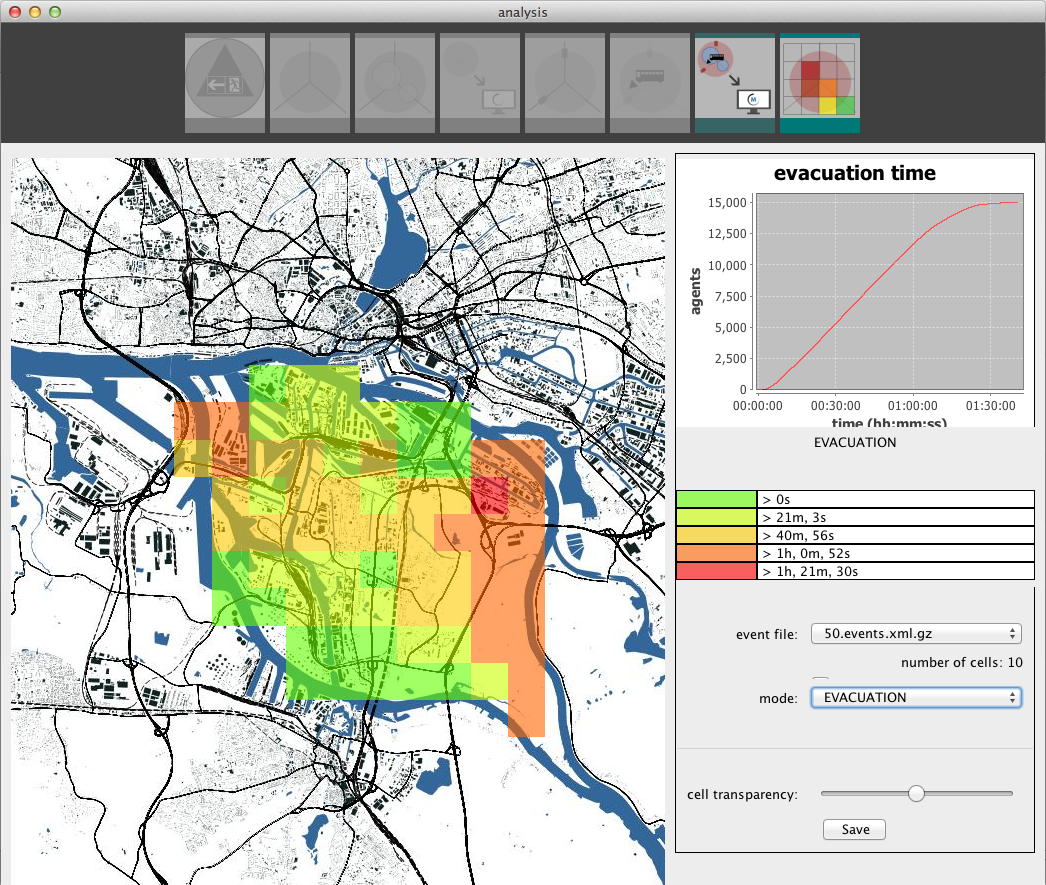
\includegraphics[width=1\textwidth]{extending/figures/Evacuation/it50_evac_time}
\caption{Screenshot of the analysis module showing GIS based evacuation time analysis and the evacuation curve.}\label{chap:evac:fig:analysis}
\end{figure}


\section{Case study}
The following describes the evacuation of Hamburg-Wilhelmsburg as a case study. Wilhelmsburg was severely flooded in 1962. Since then, many structural and operational improvements have been implemented. Back then, the housing situation was rather bad, many people lived in provisional housing due to destruction in World War II. Additionally to the by far more stable buildings, precautions for flooding have been taken and the walls have been heightened. Evacuation is nevertheless necessary under certain circumstances. The relocation of one of the major roads in Wilhelmsburg, the B75, will also influence the evacuation traffic, since it is one of the major north-south arterial roads. In this case study, the consequences of this relocation on the evacuation of Hamburg-Wilhelmsburg is investigated.
% !TeX spellcheck = en_US
% !TeX encoding = UTF-8
% !TeX program = pdflatex
% !TeX bib = biber

%\section{Case study}
%\todo{case study HH-Willhelmsburg}
%\input{casestudy.ltx}

\subsection{Brief Description}

The scenario to be investigated here is the relocation of the highway B75 in Wilhelmsburg. 
Two cases were investigated, as summarized in the following table.

\begin{table}[!ht]
\caption{Scenarios.}
\label{table:b75scenarios}
\begin{tabular}{|l | l|}
\hline
1 & Current location of B75 with restricted directional choice\\
2 & New location of B75 with restricted locational choice\\
\hline
\end{tabular}
\end{table}

\begin{figure}[!ht]
	\centering
	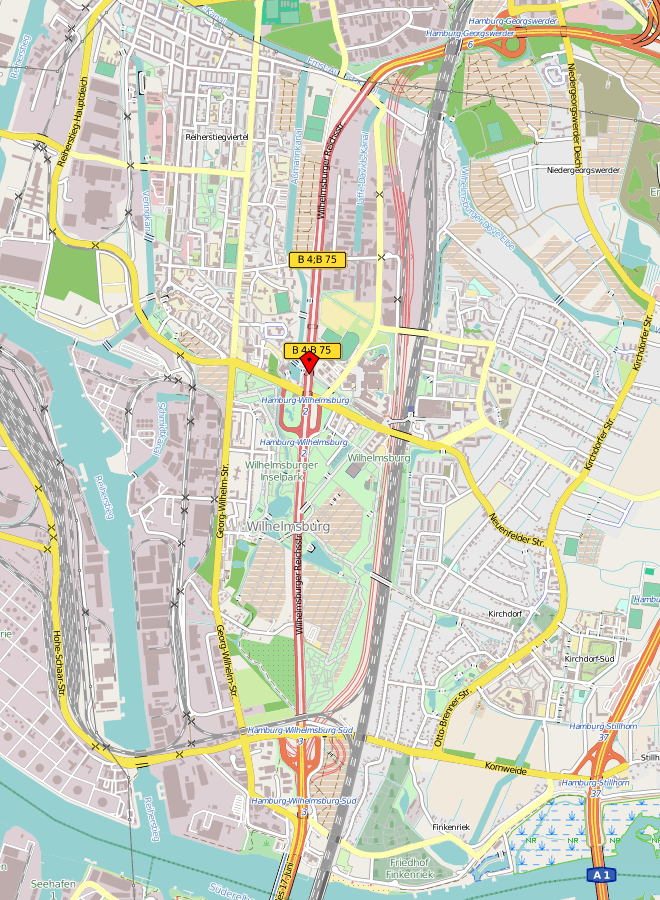
\includegraphics[width=0.7\linewidth]{extending/figures/Evacuation/B75overview}
	\caption[New and old section of B75]{The current trail of highway B75 is shown in the center of the image. The new trails is east of it close to the railroad.}
	\label{fig:overviewB75}
\end{figure}

The aim of the investigation is to highlight differences in the evacuation traffic for both variants of the B75 trail. As can bee seen from fig.~\ref{fig:overviewB75} the new trail "B75 new" is mainly located next to the existing railway track.
In the south, the new variant is connected to the existing highway at the junction "Hamburg Wilhelmsburg S\"ud" (just north of the bridge across the river Elbe) and in the north it is connected to the existing highway just before the junction "Hamburg Georgswerder". 
The main differences between the two variants ar the access to the highway B75 in the center of Wilhelmsburg.

\subsection{Road network}
The MATSim road network is generated ("imported") from the Hamburg OSM-file. This file was downloaded from \url{www.geofabrik.de}. Fortunately, the osm-file already contains the new track of the B75 highway, marked by an attributed "open 2016". Therefore, the two networks for the variants "B75 old" and "B75 new" can be derived from the same osm-file. For the variant "B75 old" this file can be directly imported. For the variant "B75 new" the part of the B75 that will be relocated, was removed in a first step. In a second step, the new B75 track was connected to the existing road network, i.e. the B75 north at junction "Georgswerder" in the north and junction "Hamburg Wilhelmsburg S\"ud" in the south.

Additionally, the internal on and off-ramps to the B75 were added. The tow variants of the resulting road network, i.e. "B75 old" and "B75 new" are shown in figure~\ref{fig:b75oldnew}.

\begin{figure}[!ht]
	\begin{subfigure}
		\centering
		\includegraphics[width=.475\linewidth]{extending/figures/Evacuation/b75old}
	\end{subfigure}\hfill
	\begin{subfigure}
		\centering
		\includegraphics[width=.475\linewidth]{extending/figures/Evacuation/b75new}
	\end{subfigure}
	\caption{Comparison between network for the old and new track of the B75.}
	\label{fig:b75oldnew}
\end{figure}

In case of an evacuation, some of the roads will be blocked. The rationale behind this is the avoidance of intersecting traffic. Furthermore, inbound traffic will be blocked, too.
The following streets are therefore deleted in the osm file:
\begin{itemize}
	\item Neuenfelder Str. 
	\item Im Sch\"onenfelde
	\item Elsterweide
	\item Kirchdorfer Str.
\end{itemize}
This is illustrated in figure~\ref{fig:b75sperrung}.
\begin{figure}
	\centering
	\includegraphics[width=0.7\linewidth]{extending/figures/Evacuation/b75sperrung}
	\caption{Roads closed during evacuation.}
	\label{fig:b75sperrung}
\end{figure}

\subsection{Evacuation Scenario}
The comparison of the two different variants is based on the overall evacuation time, the clearing time of different cells (squares in the area that has to be evacuated), and the numbers of cars using the road network (utilization).

As described in the previous section \ref{evac:section:fifteenminute}, the input files for the network (osm), the area (shp), and the population (shp) as well as the parameters for sample size and departure time distribution can be specified and assessed via the GUI. They are stored in an XML file. The scenario-xml-file for the existing (or "old", in German "alt") track of the B75 highway is shown in the following listing. 

\lstinputlisting[language=XML]{extending/modules/whb_B75alt.xml}

\subsubsection{Departure Time Distribution}
The departure time distribution is specified in the file scenario.xml. The values are in seconds, i.e. a normal distribution with a mean value (mu) and a standard deviation (sigma) of 30 minutes in the range of zero (earliest) to one hour (latest) is chosen. 
More details on the topic of time distributions can be found in section~\ref{chap:evac:eq:mu}. This distribution reflects some assumptions made concerning the evacuation procedure. The overall time frame based on the warning time is 7 hours at minimum. The preparation phase takes three hours, two hours for setting the buses up and alarming the emergency staff and one hour for the boarding of the buses. The available time for the evacuation is three hours with a buffer of one hour. 
The warning via radio is started at t=0 hrs and the local warning (e.g., by police cars, sirens, and via short messages) at t=1 hrs. Therefore, the reference point for our simulation was set to t=3 hrs. The acceptance criterion for the simulation concerning overall time is the required safe evacuation time (for the sake of the simulation by car) to be less than three hours (including reaction time). The reaction time set in the simulation can therefore be interpreted as a decision making time after having prepared the personal belongings. In short: ASET (available safe evacuation time determined by the flooding) is 3 hours and the required safe egress time is determined by the simulation. The criterion for a successful evacuation is ASET > RSET.

\subsubsection{Population Size}
As explained previously, the population size is not stored in the scenario file but in the population shape file. The reason is that a population file might consist of several polygons and the number of persons is an attribute to that polygon. In our case, the population size is 11,924 agents. This number was derived from the number of cars registered in Wilhelmsburg. There is an overall population of approximately 50,000. One has to take into account the fact, that only part of the population will have to evacuate. For many, it might be sufficient to go to higher places. Detailed information on the different procedures can be found at \url{http://www.hamburg.de/sturmflut/3425646/sturmflut-download-1/} (in German, though).

Each agent represents a car. If you would like to check the number of agents yourself based on the simulation files, you can open the file population.dbf with your database or spreadsheet editor. Please note that the number specified in the population.shp (resp. population.dbf) will be multiplied with the sampleSize when converting the files to MATSim input, i.e. in this case the population.xml.gz located in the <outputDir>.

The population is initially distributed as shown in figure~\ref{fig:b75initial}. 

\begin{figure}[th!]
\centering
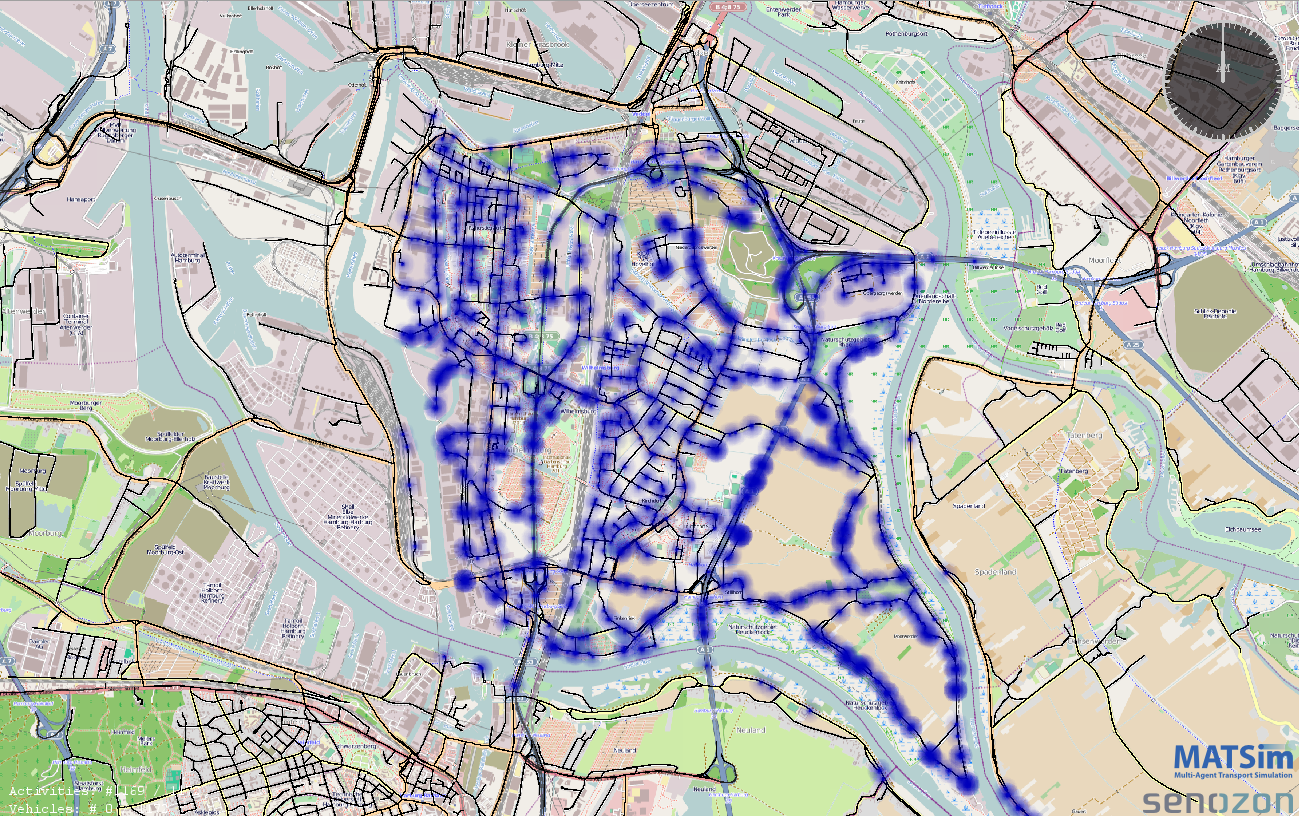
\includegraphics[width=0.7\linewidth]{extending/figures/Evacuation/B75initial}
\caption[Initial Distribution of Agents.]{The initial distribution of the agents for the evacuation of Wilhelmsburg (for both cases, B75 new and old).}
\label{fig:B75initial}
\end{figure}

The algorithm that converts the area and the population (i.e. area.shp and population.shp) is described in \ref{chap:evac:fig:area_pop}). It assigns agents to the edges of the network. For our case, the areas of the harbor were left out and agents were equally distributed to the streets of the housing (and agricultural) areas of Wilhelmsburg (cf. fig.~\ref{fig:B75initial}).
This could of course be further refined by going to blocks or even houses and assigning the population according to the detailed statistical housing data. This was not performed for the sake of this simulation, though. The main reason is twofold: Firstly, there are many assumptions concerning the behavior, initial location, and share of population that needs to evacuate. Therefore, the level of detail seems to be sufficient. Secondly, each agent represents a car, i.e. in the simulation all the cars registered in Wilhelmsburg leave the area. Taking into account the fact that inbound and through traffic will be prohibited when the level of flooding exceeds a certain threshold, this is a "worst case" assumption leading the a rather heavy traffic load. In summary, the overall approach seems to be justified to assess the relocation of the highway B75 based on a rather heavy traffic load with a reaction time span between 0 and 1 hour.

\subsection{Simulation Results}

The simulation results are summarized in table~\ref{table:b75results}. The 0th iteration is based on the shortest distance only. 

\begin{table}[!ht]
	\centering
	\caption{Results.}
	\label{table:b75results}
\begin{tabular}{|c|c|c|}
	\hline \rule[-2ex]{0pt}{5.5ex}  & B75 old & B75 new \\ 
	\hline \rule[-2ex]{0pt}{5.5ex}  Iteration & Time &  (hh:mm) \\ 
	\hline \rule[-2ex]{0pt}{5.5ex}  00 & 04:45 &  05:00\\ 
	\hline \rule[-2ex]{0pt}{5.5ex}  10 & 01:52 &  01:58\\ 
	\hline \rule[-2ex]{0pt}{5.5ex}  20 & 01:42 &  01:46\\ 
	\hline \rule[-2ex]{0pt}{5.5ex}  30 & 01:40 &  01:42\\ 
	\hline 
\end{tabular} 
\end{table}

For iteration 0, the all agents take the shortest routes. This might result in "strange" behavior as illustrated in the following figure~\ref{fig:B75iteration0}.
South of the bridge across the Elbe river, near the junction "Gro{\ss}moordamm". The road network has a circular shape resulting from the fact that it is cut out from the osm road network according to the area.shp which is in our case just a circle. Since all the agents are taking the shortest path in iteration 0, they area heading to the closest road out of the evacuation area. Technically, the boundary links in the network are connected to a super link when creating the MATSim network from the osm-file and the area.shp. This super-link or evacuation node is the destination in all evacuees plans. 

\begin{figure}[th!]
\centering
\includegraphics[width=0.7\linewidth]{extending/figures/Evacuation/b75iteration0}
\caption[Results for B75 old, iteration 0.]{Results for B75 old, iteration 0.}
\label{fig:B75iteration0}
\end{figure}

A second factor contributing to the congestion in iteration 0 is a short cut via an on- and off-ramp of the Autobahn A253 at "Gro{\ss}moordamm". The capacity of the on- and off-ramp is 1,500 cars per hour compared to 4,000 cars per hour on the highway. Therefore, the short cut (which is shorter in distance, that's the reason why the agents take it) is a bottleneck, resulting in artificial congestion in iteration 0.
Therefore, the 0th iteration is not suitable for assessing the overall evacuation time. As can be seen from table~\ref{table:b75results} above, for both cases, from iteration 10 on the time presumably converges to some realistic value. This is also illustrated in figure~\ref{figure:b75iteration20} where the situation at t=1:30 hrs is shown for iteration 20.

\begin{figure}
\centering
\includegraphics[width=0.7\linewidth]{extending/figures/Evacuation/B75iteration20}
\caption{Results for B75 old, iteration 20.}
\label{fig:B75iteration20}
\end{figure}


In summary, the relocation of the highway B75 has no major influence on the overall evacuation time. The evacuation time of about 2 hours is also within the range of the available safe egress time as described in the previous section. 

Finally, it is of course possible to analyze the results further. The two screenshots above for the situation in iteration 0 at t=3 hours and for iteration 20 at t=1.5 hours have been produced by the visualizer senozon Via.
As a conclusion to this chapter and an illustration for the built-in capabilities of Grips for analyzing simulation results, we finally show the road utilization of the two variants in figure~\ref{fig:b75utilization}.

\begin{figure}[!ht]
	\begin{subfigure}
		\centering
		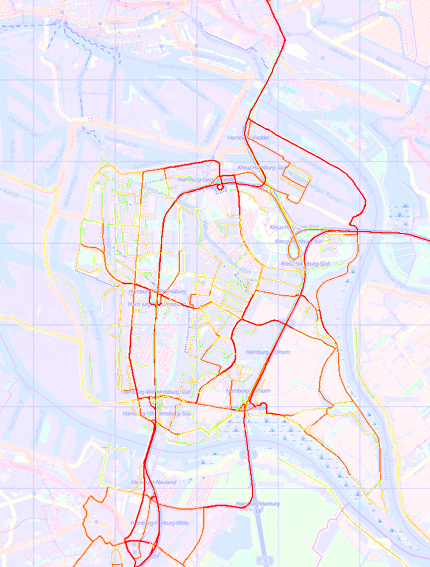
\includegraphics[width=.475\linewidth]{extending/figures/Evacuation/b75utilizationold}
	\end{subfigure}\hfill
	\begin{subfigure}
		\centering
		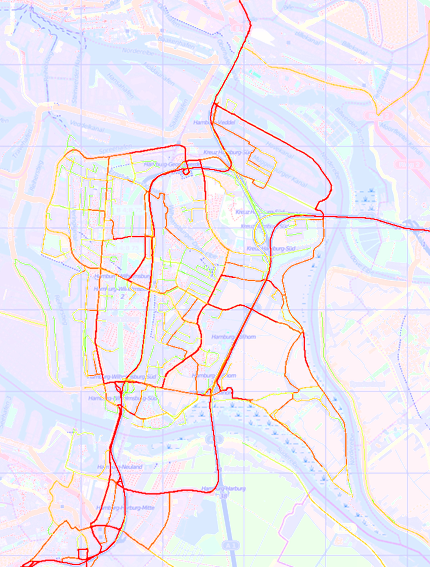
\includegraphics[width=.475\linewidth]{extending/figures/Evacuation/b75utilizationnew}
	\end{subfigure}
	\caption{Comparison between network utilization for the old and new track of the B75.}
	\label{fig:b75utilization}
\end{figure}



